\section{Identification and Removal of Code Inefficiencies}
\label{identification}

Inefficiency removal is a two stage iterative process. First, the code must be analysed to identify the critical sections of the code that take the most time executing. This can process can be automatised by using third party tools, such as gprof or callgrind, which produce a report listing the percentage of time spent in each of the application functions. A more detailed analysis can be obtained using tools similar to PAPI, where hardware counters are measured to obtain cache miss rates, float point instructions, and other low level information.

The test environment used in both this section and section \ref{removal} is a dual-socket system with two Intel E5-2670v2 with 10 cores (20 hardware threads) at 2.5 GHz each, 256 KB L2 cache per core and 25 MB shared L3 cache, coupled with 64 GB DDR3 RAM.

\subsection{First Iteration}

In a preliminary analysis using callgrind, we identified the \ttDilepKinFit as the most time consuming function when considering a significant number of variations, as shown in figure \ref{fig:ttDilepKinFit}. One particularity was that the Pseudo-Random Number Generator (PRNG) seed was being reset for every variance applied to the particles parameters, consuming XXX for 512 variations.

\begin{figure}[!htp]
	\begin{center}
		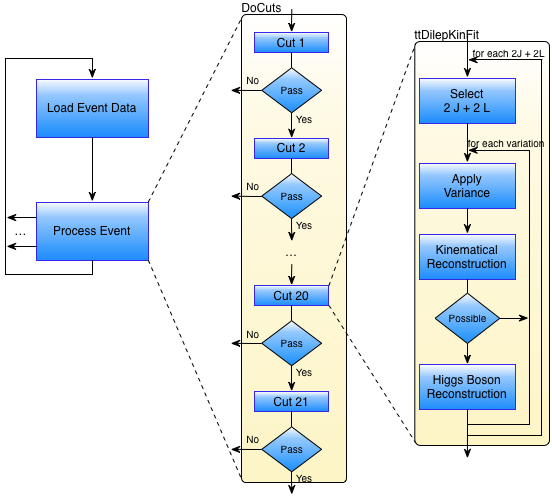
\includegraphics[scale=0.4]{images/graf_abstract_flow_with_kinfit.png}
		\caption{Schematic representation for the \tth application flow.}
		\label{fig:ttDilepKinFit}
	\end{center}
\end{figure}

Since the period of the Mersenne Twister, which is the PRNG used, is approximately $4.3 * 10^6001$ and the maximum amount of generated numbers in the input test file used, for this amount of variations, is $1.5 * 10^9$, it is not necessary to reset the seed. The removal of this simple inefficiency granted speedups up to 1.8, as shown in figure \ref{fig:PRNG}. Note that there are not tests for 1024 variations as the application execution time rendered them infeasible.

\begin{figure}[!htp]
	\begin{center}
		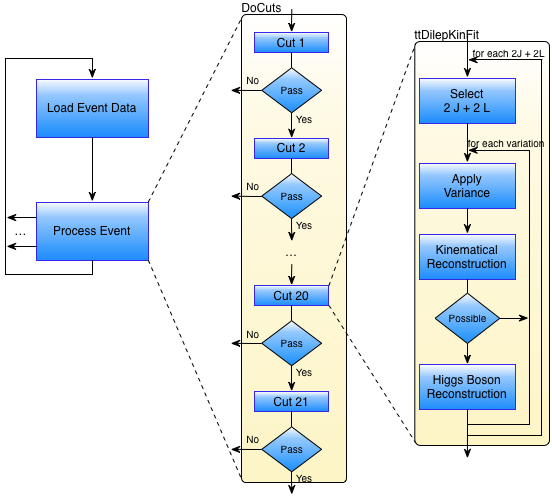
\includegraphics[scale=0.4]{images/graf_abstract_flow_with_kinfit.png}
		\caption{Schematic representation for the \tth application flow.}
		\label{fig:PRNG}
	\end{center}
\end{figure}

\subsection{Second Iteration}

Even with the PRNG optimization the \ttDilepKinFit remains the critical region in the application. Since there are no relevant code inefficiencies left the next step is to parallelize \ttDilepKinFit. Keep in mind that it is not possible to parallelize the whole event processing since part of its information is stored in LipMiniAnalysis library, which we did not have permission to refactor.

Parallelization of \ttDilepKinFit implies modifying its flow. The data of each variation is overwritten for each different combination of an event, so it is needed to create a data structure of all combinations of the event being processed. Picking the lepton/jets combination depends on all previous combinations, which serializes the construction of the data structure. Each parallel task (indivisible work segment) picks a combination with variations still to compute, varies the particles parameters and performs the kinematical and (if possible) Higgs reconstruction. Then, since only the most accurate reconstruction must be considered, a parallel merge is performed. Figure \ref{fig:SeqPipeline} presents the sequential and parallel workflow for \ttDilepKinFit.

\begin{figure}[!htp]
	\begin{center}
		\raisebox{-0.5\height}{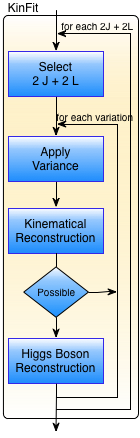
\includegraphics[scale=0.7]{images/sequential_kinfit.png}}
		\raisebox{-0.5\height}{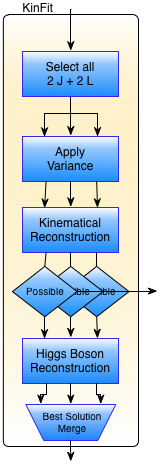
\includegraphics[scale=0.7]{images/parallel_kinfit.png}}
		\caption{Schematic representation of the \ttDilepKinFit sequential (left) and parallel (right) workflows.}
		\label{fig:SeqPipeline}
	\end{center}
\end{figure}

The parallelization was performed using OpenMP. The parallel tasks are grouped into threads, which holding the data of the best reconstruction to minimize the complexity of the best reconstruction merge by reducing through all the threads instead of tasks. The amount of tasks for each thread is balanced dynamically by the OpenMP scheduler. Each thread has a private PRNG initialized with different seeds to avoid correlation between the numbers generated.

Figure \ref{fig:non_pointer_speedup} presents the speedups for 

\begin{figure}[!htp]
	\begin{center}
		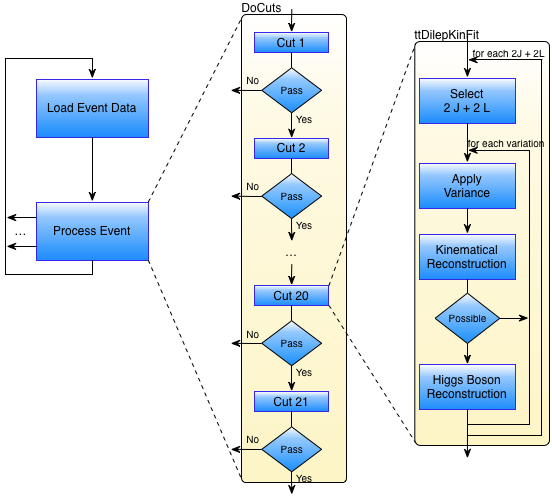
\includegraphics[scale=0.4]{images/graf_abstract_flow_with_kinfit.png}
		\caption{Speedup for \tth parallel non-pointer version application.}
		\label{fig:non_pointer_speedup}
	\end{center}
\end{figure}

\subsection{Third Iteration}

We used Intel's VTune to search for hotspots (bottlenecks) on the application, since this tool is best suited for profiling parallel applications while providing an easy to use GUI. From a preliminary analysis it was concluded that the application was spending around 20\% of the time building the combination data structure for 256 variations.

A closer look to the data structure revealed that there were inefficiencies that were affecting the performance in specific situations. There is read-only control information that is being replicated in each element of the data structure. If the elements were to share a pointer to such data the overhead of constructing the data structure would be reduced. However, this adds an increase in communication, which could lead to worse cache management and added overhead in NUMA environments. Nevertheless, this optimization was implemented and tested (addressed as \textit{pointer version}), with its speedups presented in figure \ref{fig:pointer_speedup}.

\begin{figure}[!htp]
	\begin{center}
		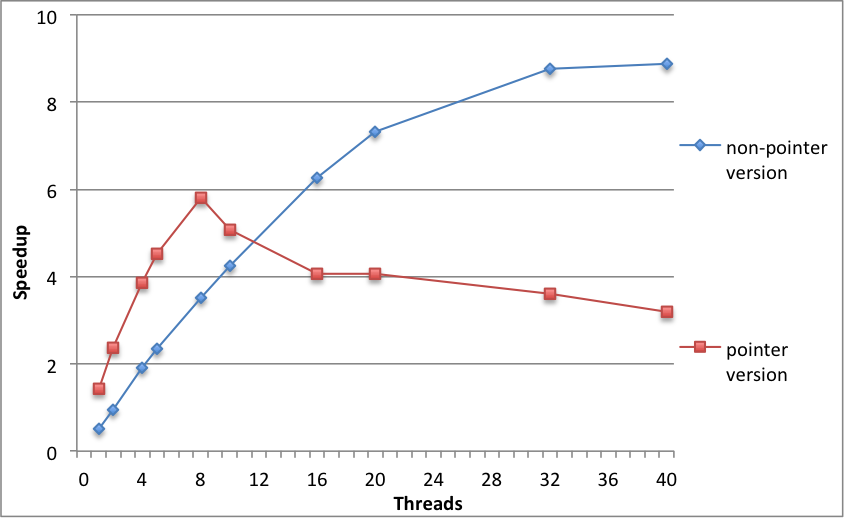
\includegraphics[scale=0.4]{charts/speedup_pointer_omp.png}
		\caption{Speedup for \tth parallel pointer version application.}
		\label{fig:pointer_speedup}
	\end{center}
\end{figure}

As predicted, the best speedup occurs when using 8 threads, which counts for almost one device on the system. Even with 10 threads the performance of the application suffers due to the increase of concurrent accesses to the L3 cache on the system due to the shared data. This decrease in performance is even more noticeable when using both CPU devices, where the non-pointer version still scales. However, this implementation is more efficient than the former when using only one device. Note that the superlinear speedups are due to the PRNG optimization and the reduction in the data that each thread has to process, making it more suitable to be stored in the private L2 cache of each core, therefore reducing the slower accesses to L3 cache.

\begin{itemize}
	\item Present MT gains?
	\item Describe the task flow with data structure?
\end{itemize}
